\section{Circuito RLC}
\begin{figure}[H]
    \centering
    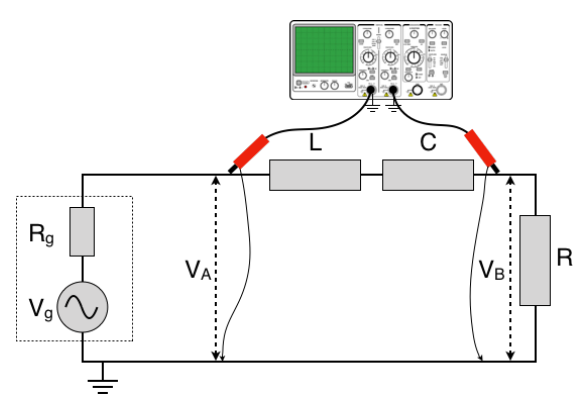
\includegraphics[scale=0.5]{Immagini/RLC.PNG}
    \caption{}
\end{figure}

Abbiamo arrangiato il circuito come in figura servendoci di una resistenza R = 1k$\Omega$.
L’obbiettivo della seconda parte dell’esperimento, similmente a prima, era lo studio della funzione di trasferimento e, attraverso il fit delle funzioni stesse, ricavare i valori dei parametri L e C.
Come in precedenza, abbiamo diviso lo studio suddividendolo in analisi del modulo e analisi della fase. 

\begin{table}[!ht]
    \centering
    \begin{tabular}{lllll}
    \toprule
         $\nu$ [Hz]  & $\omega$ & $V_a$ [V] & $V_b$ [V] & $V_{a-b}$ [V]  \\ 
         \midrule
        5  & 0,80 & 3,04 & 2,6 & 1,2  \\ 
        15  & 2,39 & 3 & 2,76 & 0,48  \\ 
        25  & 3,98 & 3,08 & 2,8 & 0,4  \\ 
        30  & 4,77 & 3,04 & 2,8 & 0,4  \\ 
        35  & 5,57 & 3 & 2,8 & 0,4  \\ 
        45  & 7,16 & 3,04 & 2,8 & 0,32  \\ 
        60  & 9,55 & 3,08 & 2,4 & 0,4  \\ 
        80  & 12,73 & 3,04 & 2,8 & 0,32  \\ 
        100  & 15,92 & 3,04 & 2,8 & 0,32  \\ 
        \bottomrule
    \end{tabular}
    \label{tabella 3}
\end{table}

Riportiamo di seguito i fit relativi ai moduli:

\begin{figure}[H]
    \centering
    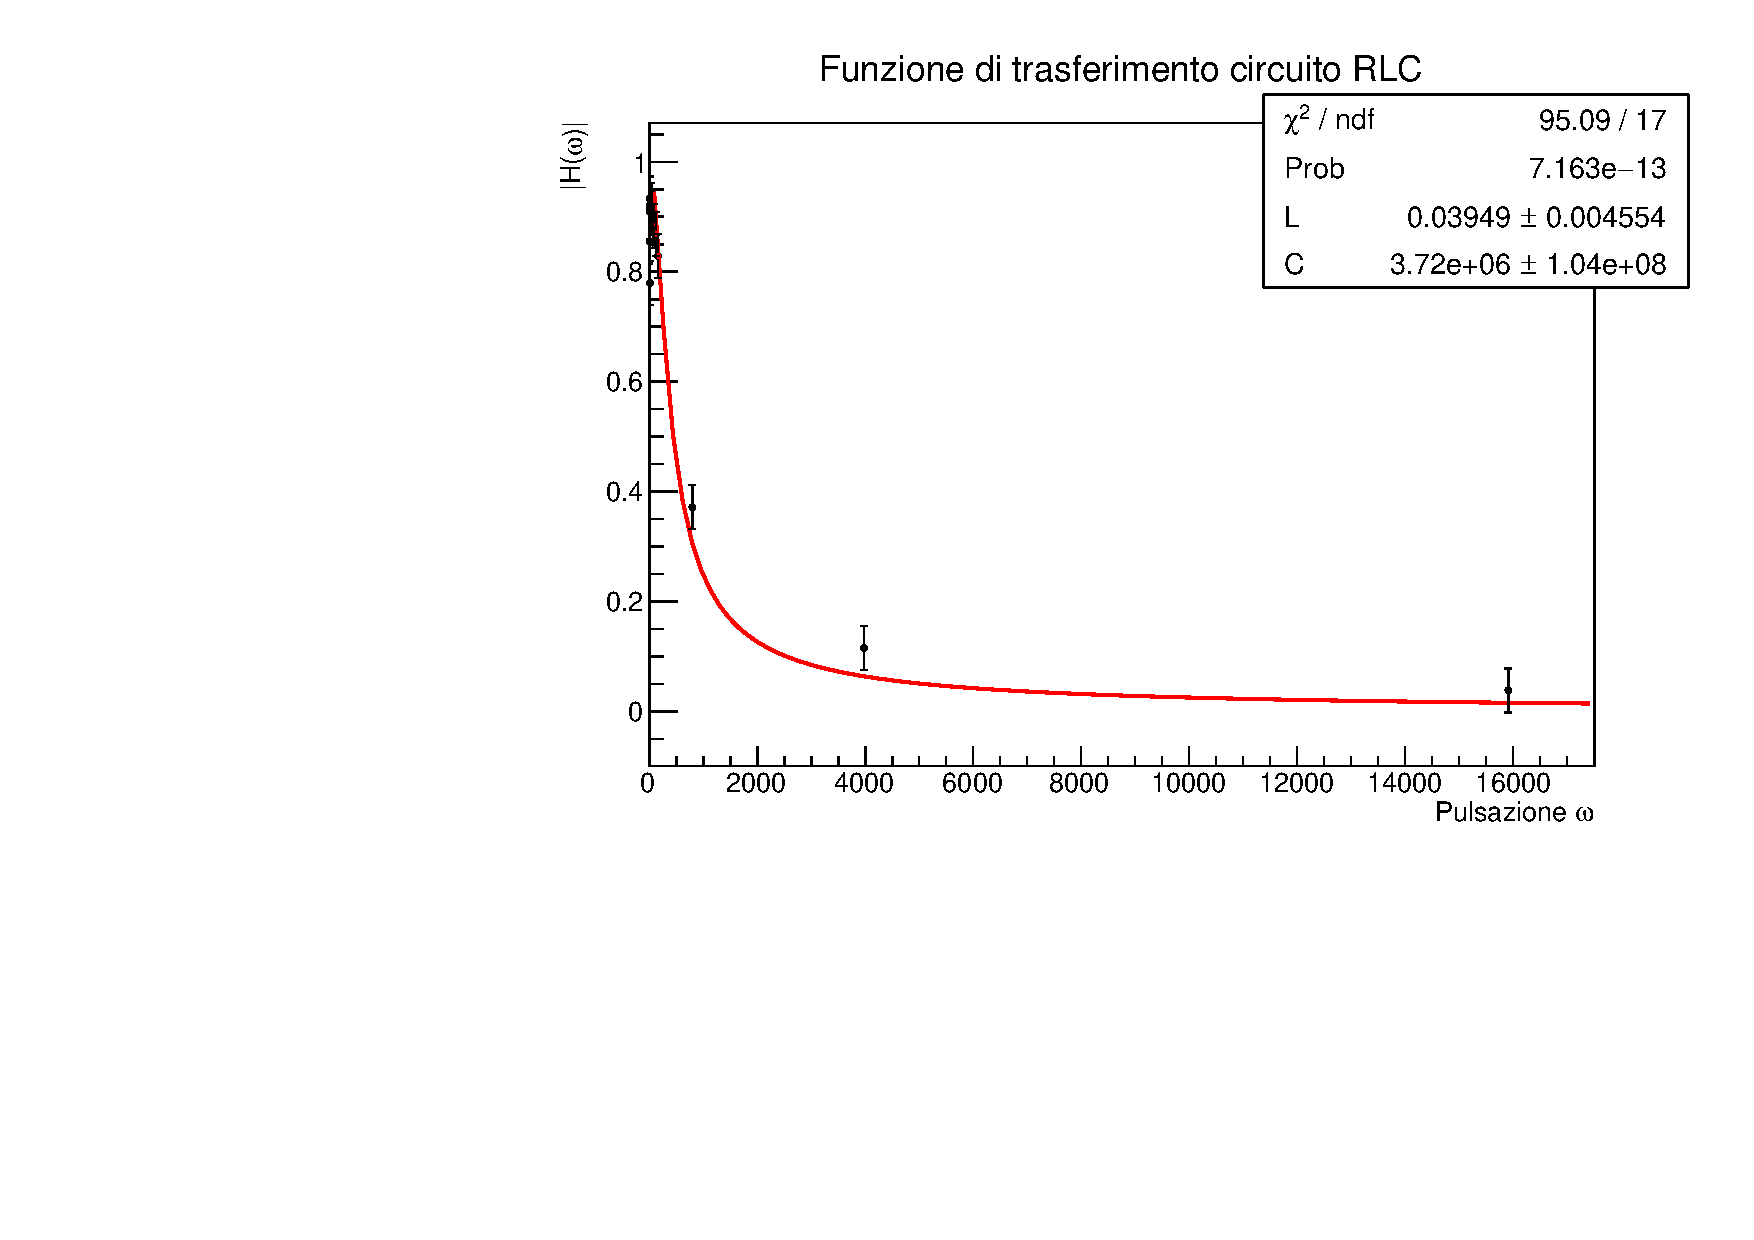
\includegraphics[scale=.4]{Immagini/trasferimento RLC.pdf}
    \\
    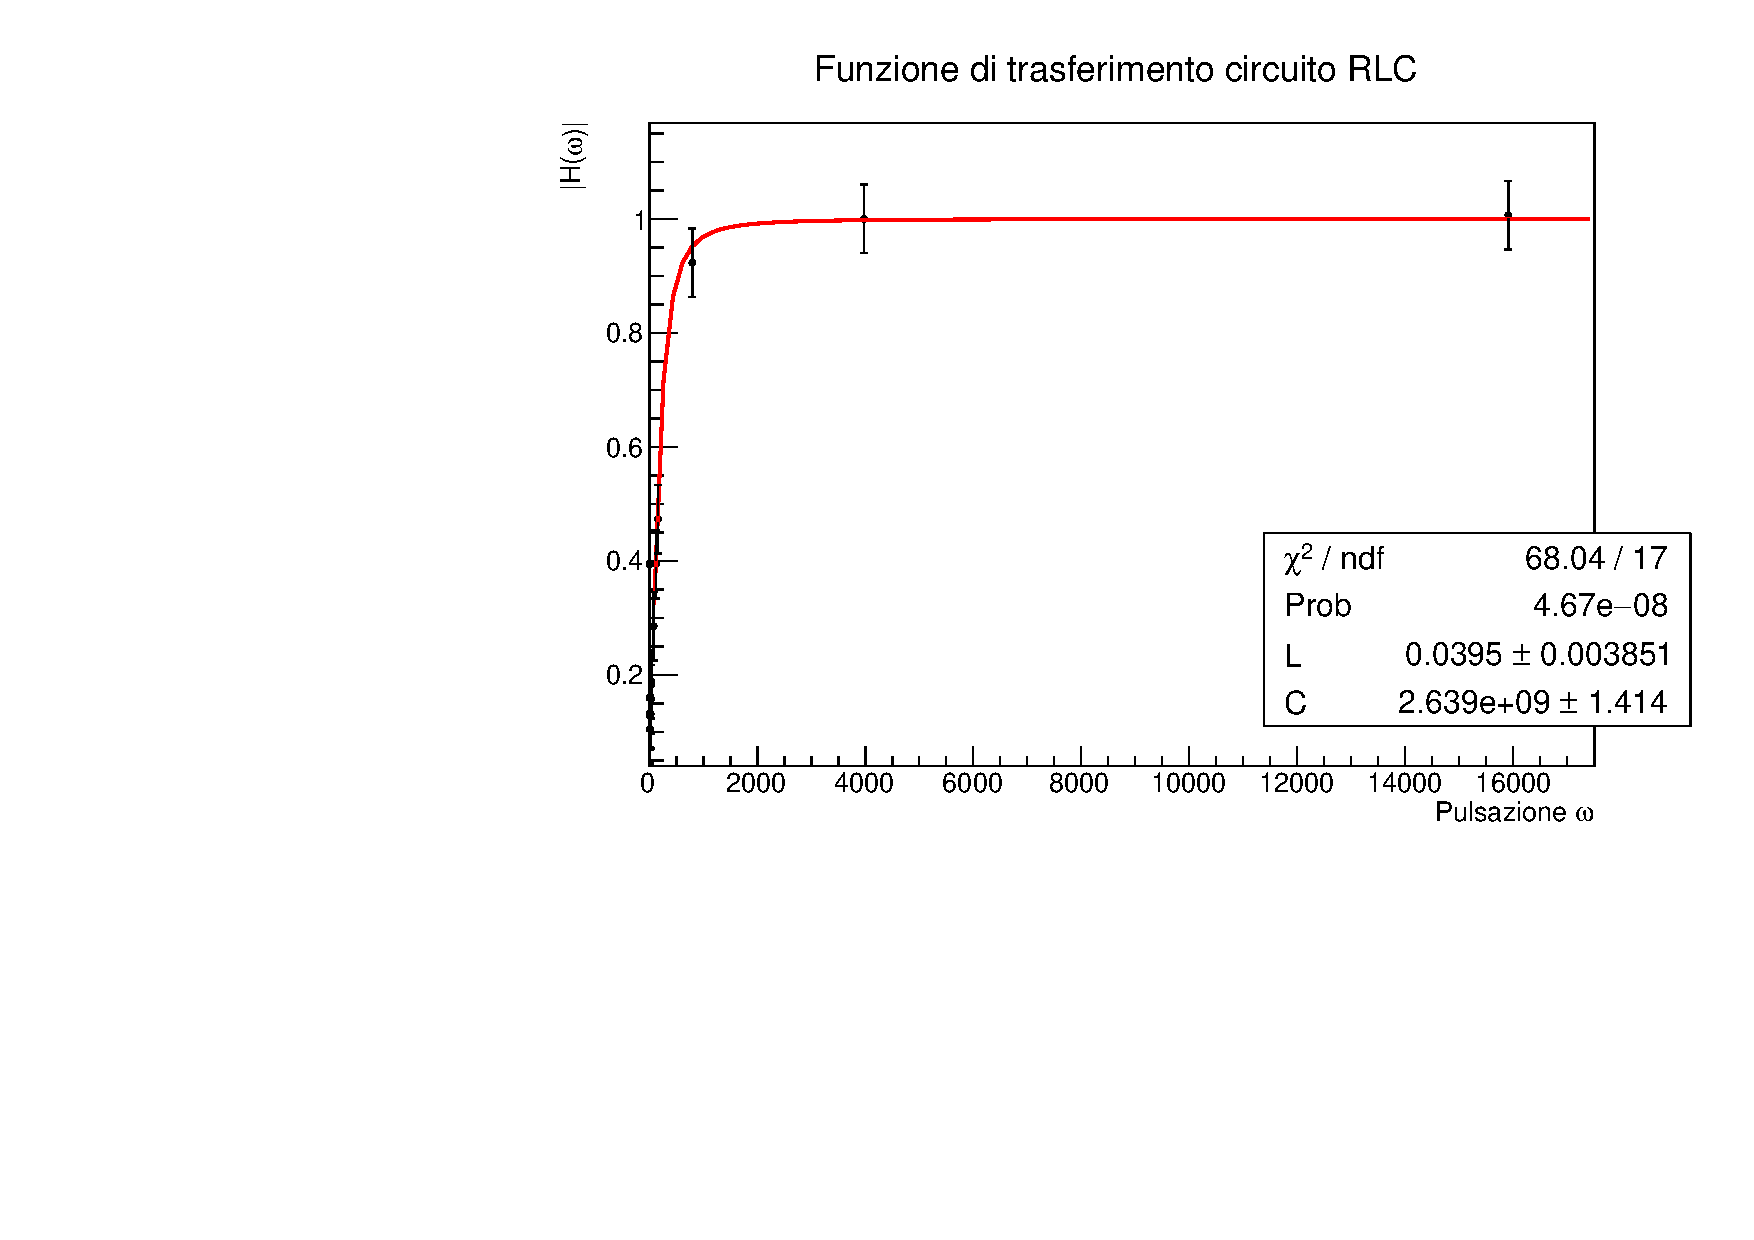
\includegraphics[scale=.4]{Immagini/trasferimento RLC 2.pdf}
    \caption{}
\end{figure}

Com'è possibile osservare dai fit presentati, i dati presentano un $\chi ^{2}$ che indica un’incompatibilità tra modello e misure raccolte, ma fornisce stime sui parametri possibili,
accettabili, in quanto dell’ordine di grandezza aspettato (decine di mHerny per l’induzione e nell’ordine dei $\mu$Farad per la capacità).

I valori di C ed L sono riportati nei grafici.

Riteniamo che il modello non venga verificato, non a causa delle misure raccolte o a causa di errori nel modello, ma a causa di un possibile mal funzionamento nell’algoritmo usato per il fit di cui non riusciamo a venire a capo. Il fit, infatti, dovrebbe riportare una funzione a campana, ma, poiché essa presenta il massimo per frequenze molto basse, anche campionando con maggior frequenza in un intorno del massimo stesso è impossibile evidenziare una crescita di ripidità comparabile con la decrescita della funzione stessa. Anche rimuovendo dei punti all’estremità destra della funzione, la crescita rimane troppo 
piccola rispetto alla decrescita e viene evidenziata, inoltre, l’oscillazione del valore del modulo della funzione di trasferimento attorno alla $\Omega$ massima portando quindi il fit a presentare incompatibilità tra modello e misure raccolte.

Come nei casi precedenti lo studio sulla fase non risulta valido.
